\documentclass{aastex62}   	% use "amsart" instead of "article" for AMSLaTeX format
\usepackage{graphicx}				% Use pdf, png, jpg, or eps§ with pdflatex; use eps in DVI mode
								% TeX will automatically convert eps --> pdf in pdflatex		
\usepackage{amssymb,amsmath}
\usepackage{natbib,verbatim}
\usepackage[multiple]{footmisc}
%\usepackage{grffile}
%\usepackage{textcase}
\usepackage{hyperref}


%\usepackage[overload]{textcase}

%SetFonts

%SetFonts

\begin{document}
%\raggedright
\begin{raggedright}
\huge
Astro2020 Science White Paper \linebreak
Testing Gravity Using Type Ia Supernovae Discovered by Next-Generation Wide-Field Imaging Surveys \linebreak
\normalsize

\noindent \textbf{Thematic Areas:} \hspace*{60pt} $\square$ Planetary Systems \hspace*{10pt} $\square$ Star and Planet Formation \hspace*{20pt}\linebreak
$\square$ Formation and Evolution of Compact Objects \hspace*{31pt} $\blacksquare$ Cosmology and Fundamental Physics \linebreak
  $\square$  Stars and Stellar Evolution \hspace*{1pt} $\square$ Resolved Stellar Populations and their Environments \hspace*{40pt} \linebreak
  $\square$    Galaxy Evolution   \hspace*{45pt} $\square$             Multi-Messenger Astronomy and Astrophysics \hspace*{65pt} \linebreak
  
\textbf{Principal Author:}

Name:	
 Alex Kim\linebreak						
Institution:  
Physics Division, Lawrence Berkeley National Laboratory, 
    1 Cyclotron Road, Berkeley, CA, 94720 \linebreak
Email:  \url{agkim@lbl.gov}
 \linebreak
Phone:  1-510-486-4621
 \linebreak
 
\textbf{Co-authors:}
%\author[0000-0001-6315-8743]{A.~G.~Kim}
%\affiliation{Physics Division, Lawrence Berkeley National Laboratory, 
%    1 Cyclotron Road, Berkeley, CA, 94720}
G.~Aldering\footnotemark[1],
\footnotetext[1]{Physics Division, Lawrence Berkeley National Laboratory, 
    1 Cyclotron Road, Berkeley, CA, 94720}
P.~Antilogus\footnotemark[2],
\footnotetext[2]{Laboratoire de Physique Nucl\'eaire et de Hautes Energies, Sorbonne Universit\'e, CNRS-IN2P3, 4 Place Jussieu, 75005 Paris, France}    
A.~Bahmanyar\footnotemark[3],
\footnotetext[3]{Department of Astronomy and Astrophysics, University of Toronto,
50 St. George Street, Toronto, Ontario, Canada M5S 3H4}
S.~BenZvi\footnotemark[4],
\footnotetext[4]{Department of Physics and Astronomy, University of Rochester, Rochester, NY 14627, USA}
H.~Courtois\footnotemark[5],
\footnotetext[5]{Universit\'e de Lyon, F-69622, Lyon, France; Universit\'e de Lyon
1, Villeurbanne; CNRS/IN2P3, Institut de Physique Nucl�aire de
Lyon, France} 
T.~Davis\footnotemark[6],
\footnotetext[6]{School of Mathematics and Physics, University of Queensland, Brisbane, QLD 4072, Australia}
S.~Gontcho A Gontcho\footnotemark[4],
%\affiliation{Department of Physics and Astronomy, University of Rochester, Rochester, NY 14627, USA}
O.~Graur\footnotemark[7]\textsuperscript{,}\footnotemark[8]\textsuperscript{,}\footnotemark[9],
\footnotetext[7]{Harvard-Smithsonian Center for Astrophysics, 60 Garden Street, Cambridge, MA 02138, USA}
\footnotetext[8]{Department of Astrophysics, American Museum of Natural History, New York, NY 10024, USA}
\footnotetext[9]{NSF Astronomy and Astrophysics Postdoctoral Fellow}
R.~Graziani\footnotemark[10],
\footnotetext[10]{Universit\'e Clermont Auvergne, CNRS/IN2P3, Laboratoire de
Physique de Clermont, F-63000 Clermont-Ferrand, France}    
C.~Harper\footnotemark[1],
%\affiliation{Physics Division, Lawrence Berkeley National Laboratory, 
%    1 Cyclotron Road, Berkeley, CA, 94720}
R.~Hlo\u{z}ek\footnotemark[3]\textsuperscript{,}\footnotemark[11],
%\affiliation{Department of Astronomy and Astrophysics, University of Toronto,
%50 St. George Street, Toronto, Ontario, Canada M5S 3H4}
\footnotetext[11]{Dunlap Institute for Astronomy and Astrophysics, University of Toronto, ON, M5S 3H4}
C.~Howlett\footnotemark[12],
\footnotetext[12]{International Centre for Radio Astronomy Research, The University of Western Australia, Crawley, WA 6009, Australia}
D.~Huterer\footnotemark[13],
\footnotetext[13]{Department of Physics, University of Michigan, 450 Church Street, Ann
Arbor, MI 48109, USA }
C.~Ju\footnotemark[12],
%\affiliation{Physics Division, Lawrence Berkeley National Laboratory, 
%    1 Cyclotron Road, Berkeley, CA, 94720}
P.-F.~Leget\footnotemark[14],
\footnotetext[14]{Laboratoire de Physique Nucl\'eaire et de Hautes Energies, Sorbonne Universit\'e, CNRS-IN2P3, 4 Place Jussieu, 75005 Paris, France}    
E.~V.~Linder\footnotemark[1],
%\affiliation{Physics Division, Lawrence Berkeley National Laboratory, 
%    1 Cyclotron Road, Berkeley, CA, 94720}
P.~McDonald\footnotemark[1],
%\affiliation{Physics Division, Lawrence Berkeley National Laboratory, 
%    1 Cyclotron Road, Berkeley, CA, 94720}
J.~Nordin\footnotemark[15],
\footnotetext[15]{Institut fur Physik, Humboldt-Universitat zu Berlin, Newtonstr. 15, 12489 Berlin, Germany}
P.~Nugent\footnotemark[16],
\footnotetext[16]{Computational Research Division, Lawrence Berkeley National Laboratory, 
    1 Cyclotron Road, Berkeley, CA, 94720}
S.~Perlmutter\footnotemark[1],
N.~Regnault\footnotemark[14],
%\affiliation{Laboratoire de Physique Nucl\'eaire et de Hautes Energies, Sorbonne Universit\'e, CNRS-IN2P3, 4 Place Jussieu, 75005 Paris, France}    
M.~Rigault\footnotemark[5],
%\affiliation{Universit\'e de Lyon, F-69622, Lyon, France; Universit\'e de Lyon
%1, Villeurbanne; CNRS/IN2P3, Institut de Physique Nucl�aire de
%Lyon, France} 
A.~Shafieloo\footnotemark[17],
\footnotetext[17]{Korea Astronomy and Space Science Institute, Yuseong-gu, Daedeok-daero 776, Daejeon 34055, Korea}
A.~Slo\u{z}ar\footnotemark[18],
\footnotetext[18]{Brookhaven National Laboratory, Physics Department, Upton, NY
11973, USA} 
M.~Wood-Vasey\footnotemark[19]
\footnotetext[19]{PITT PACC, Department of Physics and Astronomy, University of Pittsburgh, Pittsburgh, PA 15260, USA} 
\linebreak

\textbf{Endorsers:}
 Behzad Ansarinejad $^{1,2}$, 
 Robert Armstrong $^{}$, 
 Carlo Baccigalupi $^{3,4,5}$, 
 Maciej Bilicki $^{6}$, 
 Julian Borrill $^{7}$, 
 Simone Ferraro $^{7}$, 
 Llu\'is Galbany $^{8}$, 
 Juan Garc\'ia-Bellido $^{9}$, 
 Juan Garc\'ia-Bellido $^{10}$, 
 Martina Gerbino $^{}$, 
 Mandeep S.S. Gill $^{11,12,13}$, 
 Larry Gladney $^{14}$, 
 Marc Kamionkowski $^{1,19}$, 
 Kazuya Koyama $^{20}$, 
 Michele Liguori $^{21}$, 
 Joel Meyers $^{22}$, 
 "Surhud More" $^{23}$, 
 Jeffrey A. Newman $^{8}$, 
 Gustavo Niz $^{24}$, 
 "Antonella Palmese" $^{25}$, 
 Francesco Piacentini $^{26}$, 
 Francesco Piacentni  $^{26,27}$, 
 Steven Rodney $^{28}$, 
 Benjamin Rose $^{29}$, 
 Lado Samushia $^{30}$, 
 Neelima Sehgal $^{31}$, 
 Leonardo Senatore $^{11}$, 
 Huanyuan Shan $^{1,33}$, 
 Scott Watson $^{35}$, 
 Martin White $^{36,7}$, 
 Weishuang Xu $^{37}$, 
 Gong-Bo Zhao $^{38,39,20}$
  \linebreak

%%% 
%\input{/Users/akim/project/AstroInstitutions/institutionAliases.tex}
% $^{1}$ \ED \\
%$^{2}$ \Durham \\
%$^{3}$ \SISSA \\
%$^{4}$ \IFPU \\
%$^{5}$ \INFN \\
%$^{6}$ \CFT \\
%$^{7}$ \LBL \\
%$^{8}$ \Pitt \\
%$^{9}$ \IFT \\
%$^{10}$ \UAM \\
%$^{11}$ \KIPAC \\
%$^{12}$ \Stanford \\
%$^{13}$ \SLAC \\
%$^{14}$ \Yale \\
%$^{15}$ \UR \\
%$^{16}$ \dunlap \\
%$^{17}$ \daa \\
%$^{18}$ \Umich \\
%$^{19}$ \JHU \\
%$^{20}$ \Port \\
%$^{21}$ \UNIPD \\
%$^{22}$ \SMU \\
%$^{23}$ \IUCAA \\
%$^{24}$ \UGTO \\
%$^{25}$ \FNAL \\
%$^{26}$ \RomaS \\
%$^{27}$ \INFNRM \\
%$^{28}$ \USC \\
%$^{29}$ \STSCI \\
%$^{30}$ \KSU \\
%$^{31}$ \StonyBrook \\
%$^{32}$ \KASSI \\
%$^{33}$ \SHAO\\
%$^{34}$ \BNL \\
%$^{35}$ \Syracuse \\
%$^{36}$ \UCB \\
%$^{37}$ \HarvardPhys \\
%$^{38}$ \NAOC \\
%$^{39}$ \UCAS \\
%
\textbf{Abstract:}
In the upcoming decade cadenced wide-field imaging surveys 
will increase the number of identified  $z<0.3$ Type~Ia supernovae (SNe~Ia)  from the hundreds to the
hundreds of thousands.  The increase in the number density  and solid-angle coverage 
of SNe~Ia, in parallel with improvements in the standardization of
their absolute magnitudes, now make them competitive probes of the growth of structure and hence of gravity.  The peculiar velocity power spectrum
is sensitive to $\gamma$, which captures the effect of gravity on the linear growth of structure through the relation $f=\Omega_M^\gamma$.
In the next decade the peculiar velocities of
SNe~Ia in the local $z<0.3$ Universe will provide a measure of $\gamma$ with as low as
$0.01$ precision that can definitively distinguish  between General Relativity and leading models of alternative gravity.
\end{raggedright}
\pagebreak
\newpage
\setcounter{page}{0}
\pagenumbering{arabic}
\setcounter{page}{1}
%\title{Testing Gravity Using Type Ia Supernovae Discovered by Next Generation Wide Field Imaging Surveys}
%\author[0000-0001-6315-8743]{A.~G.~Kim}
%\affiliation{Physics Division, Lawrence Berkeley National Laboratory, 
%    1 Cyclotron Road, Berkeley, CA, 94720}
%\author{G.~Aldering}
%\affiliation{Physics Division, Lawrence Berkeley National Laboratory, 
%    1 Cyclotron Road, Berkeley, CA, 94720}
%\author{P.~Antilogus}
%\affiliation{Laboratoire de Physique Nucl\'eaire et de Hautes Energies, Sorbonne Universit\'e, CNRS-IN2P3, 4 Place Jussieu, 75005 Paris, France}    
%\author{A.~Bahmanyar}
%\affiliation{Department of Astronomy and Astrophysics, University of Toronto,
%50 St. George Street, Toronto, Ontario, Canada M5S 3H4}
%\author{S.~BenZvi}
%\affiliation{Department of Physics and Astronomy, University of Rochester, Rochester, NY 14627, USA}
%\author{H.~Courtois}
%\affiliation{Universit\'e de Lyon, F-69622, Lyon, France; Universit\'e de Lyon
%1, Villeurbanne; CNRS/IN2P3, Institut de Physique Nucl�aire de
%Lyon, France} 
%\author{T.~Davis}
%\affiliation{School of Mathematics and Physics, University of Queensland, Brisbane, QLD 4072, Australia}
%\author{S.~Gontcho A Gontcho}
%\affiliation{Department of Physics and Astronomy, University of Rochester, Rochester, NY 14627, USA}
%\author{O.~Graur}
%\affiliation{Harvard-Smithsonian Center for Astrophysics, 60 Garden Street, Cambridge, MA 02138, USA}
%\affiliation{Department of Astrophysics, American Museum of Natural History, New York, NY 10024, USA}
%\affiliation{NSF Astronomy and Astrophysics Postdoctoral Fellow}
%\author{R.~Graziani}
%\affiliation{Universit\'e Clermont Auvergne, CNRS/IN2P3, Laboratoire de
%Physique de Clermont, F-63000 Clermont-Ferrand, France}    
%\author{C.~Harper}
%\affiliation{Physics Division, Lawrence Berkeley National Laboratory, 
%    1 Cyclotron Road, Berkeley, CA, 94720}
%\author{R.~Hlo\u{z}ek}
%\affiliation{Department of Astronomy and Astrophysics, University of Toronto,
%50 St. George Street, Toronto, Ontario, Canada M5S 3H4}
%\affiliation{Dunlap Institute for Astronomy and Astrophysics, University of Toronto, ON, M5S 3H4}
%\author{C.~Howlett}
%\affiliation{International Centre for Radio Astronomy Research, The University of Western Australia, Crawley, WA 6009, Australia}
%\author{D.~Huterer}
%\affiliation{Department of Physics, University of Michigan, 450 Church Street, Ann
%Arbor, MI 48109, USA }
%\author{C.~Ju}
%\affiliation{Physics Division, Lawrence Berkeley National Laboratory, 
%    1 Cyclotron Road, Berkeley, CA, 94720}
%\author{P.-F.~Leget}
%\affiliation{Laboratoire de Physique Nucl\'eaire et de Hautes Energies, Sorbonne Universit\'e, CNRS-IN2P3, 4 Place Jussieu, 75005 Paris, France}    
%\author{E.~V.~Linder}
%\affiliation{Physics Division, Lawrence Berkeley National Laboratory, 
%    1 Cyclotron Road, Berkeley, CA, 94720}
%\author{P.~McDonald}
%\affiliation{Physics Division, Lawrence Berkeley National Laboratory, 
%    1 Cyclotron Road, Berkeley, CA, 94720}
%\author{J.~Nordin}
%\affiliation{Institut fur Physik, Humboldt-Universitat zu Berlin, Newtonstr. 15, 12489 Berlin, Germany}
%\author{P.~Nugent}
%\affiliation{Computational Research Division, Lawrence Berkeley National Laboratory, 
%    1 Cyclotron Road, Berkeley, CA, 94720}\author{S.~Perlmutter}
%\affiliation{Physics Division, Lawrence Berkeley National Laboratory, 
%    1 Cyclotron Road, Berkeley, CA, 94720}
%\affiliation{Department of Physics, University of California Berkeley, 366 LeConte Hall MC 7300, Berkeley, CA, 94720-7300}
%\author{N.~Regnault}
%\affiliation{Laboratoire de Physique Nucl\'eaire et de Hautes Energies, Sorbonne Universit\'e, CNRS-IN2P3, 4 Place Jussieu, 75005 Paris, France}    
%\author{M.~Rigault}
%\affiliation{Universit\'e de Lyon, F-69622, Lyon, France; Universit\'e de Lyon
%1, Villeurbanne; CNRS/IN2P3, Institut de Physique Nucl�aire de
%Lyon, France} 
%\author{A.~Shafieloo}
%\affiliation{Korea Astronomy and Space Science Institute, Yuseong-gu, Daedeok-daero 776, Daejeon 34055, Korea}
%\author{A.~Slo\u{z}ar}
%\affiliation{Brookhaven National Laboratory, Physics Department, Upton, NY
%11973, USA} 
%\author{M.~Wood-Vasey}
%\affiliation{PITT PACC, Department of Physics and Astronomy, University of Pittsburgh, Pittsburgh, PA 15260, USA} 
%\author{others}

%\date{}							% Activate to display a given date or no date

%\begin{abstract}
%In the upcoming decade cadenced wide-field imaging surveys 
%will increase the number of identified  $z<0.3$ Type~Ia supernovae (SNe~Ia)  from the hundreds to the
%hundreds of thousands.  The increase in the number density  and solid-angle coverage 
%of SNe~Ia, in parallel with improvements in the standardization of
%their absolute magnitudes, now make them competitive probes of the growth of structure and hence of gravity.  The peculiar velocity power spectrum
%is sensitive to $\gamma$, which captures the effect of gravity on the linear growth of structure through the relation $f=\Omega_M^\gamma$.
%In the next decade the peculiar velocities of
%SNe~Ia in the local $z<0.3$ Universe will provide a measure of $\gamma$ with as low as
%$0.01$ precision that can definitively distinguish  between General Relativity and leading models of alternative gravity.
%\end{abstract}

\section{Introduction}

In the late 1990's, Type~Ia supernovae (SNe~Ia) were used as distance probes to measure the homogeneous expansion history of the Universe.  The remarkable discovery
that the expansion is accelerating  has called into question our basic understanding of the gravitational forces within the Universe.  Either it
is dominated by a ``dark energy'' that is gravitationally repulsive, or General Relativity is inadequate and needs to be replaced by a modified theory of
gravity.  It is only appropriate that in the upcoming decade, with their sheer numbers, solid-angle coverage,
and improved distance precisions, SNe~Ia will provide measurements of the {\it inhomogeneous} motions of structures in the Universe
that will provide an unmatched test of whether dark energy or modified gravity is responsible for the accelerating expansion of the Universe.

In the next decade, SNe~Ia will be used as peculiar-velocity probes to measure  the influence of gravity on structure formation within the Universe.
The SN~Ia Hubble diagram has  scatter along the redshift axis since peculiar velocities induce differing observed and cosmological redshifts.  The contribution
of this scatter is pronounced at low redshifts and when the scatter along the magnitude axis (i.e.\ intrinsic magnitude dispersion) is small.
The peculiar velocity power spectrum is sensitive to the growth of structure as $P_{vv}\propto (fD)^2$, where $D$ is  the spatially-independent
growth factor for the linear evolution of density perturbations and
$f \equiv \frac{d\ln{D}}{d\ln{a}}$ is the linear growth rate  \citep{2006PhRvD..73l3526H,2011ApJ...741...67D}.\footnote{
To be precise, the peculiar
velocity power spectrum also depends on the Hubble parameter as $P_{vv}\propto (HfD)^2$.  A supernova  survey  measures luminosity distance fluctuations
$\delta_{d_L} = (d_L- \bar{d}_L(z))/\bar{d}_L(z)$, where $d_L$ is the observed distance and $\bar{d}_L(z)$ is the expected distance at the observed redshift $z$.
To first order in peculiar velocity along the line of sight $v$, $\delta_{d_L} =  v \left(1-\frac{1}{H\bar{d}_L(z)}\right) \approx -\frac{v}{H\bar{d}_L(z)}$
at low redshift.   The $H$-dependences of  $P_{vv}$ and the conversion from distances to velocities cancel, making  peculiar velocity surveys sensitive to $(fD)^2$.
}
The $\Lambda$CDM prediction for the $z=0$ peculiar velocity power spectrum is shown in Figure~\ref{power:fig}. The growth of structure depends on gravity, indeed 
\citet{2007APh....28..481L} find that General Relativity, $f(R)$,  and DGP gravity follow the relation
$f \approx \Omega_M^\gamma$ with $\gamma=0.55, 0.42, 0.68$ respectively \citep[see][for a review of
these gravity models within a cosmological context]{HUTERER201523}.  Adopting this parameterization to model gravity, peculiar velocity
surveys are  sensitive to $fD=\Omega_M^{\gamma} \exp{\left(\int_a^1 \Omega_M^{\gamma} d\ln{a} \right)}$, whose prediction for $\Lambda$CDM  is plotted 
in Figure~2 of  \citet{1475-7516-2013-04-031}.\footnote{The parameter $\sigma_8$, the  standard deviation of overdensities in 8$h^{-1}$Mpc spheres, is 
commonly used in place of $D$ to normalize the
overall amplitude of  overdensities, so the standard parameterization used by the community is $f\sigma_8$.}


\begin{figure}
\centering
\includegraphics[width=0.47\textwidth]{src/new2.png}
%\includegraphics[width=0.5\textwidth]{../outcosmo/zmax_.png}
\caption{Volume-weighted peculiar velocity power spectrum $k^3P_{vv}(z=0)$ for $\mu=1, 0.5$ (solid black, cyan)  as predicted for General Relativity in the linear regime.
Overplotted are volume-weighted peculiar velocity shot-noise  $k^3\sigma^2/n$ at $z=0.1$ expected from 2- and 10-year (red, black) supernova densities, 0.08 and 0.15~mag (dashed, dotted) intrinsic magnitude dispersions, and TAIPAN (green, dash-dotted).
The bottom solid horizontal lines show the approximate range of $k$ expected to be used in surveys with corresponding
redshift depths $z_{max}$.
\label{power:fig}}
\end{figure}


Peculiar velocity surveys have already been  used to measure $fD$, though not to a level where  gravity models can be precisely distinguished.
 \citet{2017MNRAS.471..839A} use 6dFGS peculiar velocities using the Fundamental Plane distances of spiral galaxies, using absolute magnitudes
 with
 $\sim 0.43$~mag  precision calibrated by emission line velocity dispersions, to
get a 15\% uncertainty in $fD$ at $z\approx 0$ using combined density and velocity information.
The upcoming 
TAIPAN survey \citep{2017PASA...34...47D} will obtain Fundamental Plane galaxies with densities of $n_g \sim 10^{-3}h^3$\,Mpc$^{-3}$,
and the WALLABY+WNSHS surveys \citep{2008ExA....22..151J} will obtain Tully-Fisher distances (based on the $\sim 0.48$~mag calibration of absolute magnitude based on the  HI 21cm line width)
of galaxies with densities $n_g \sim 2\times 10^{-2} - 10^{-4} h^3$\,Mpc$^{-3}$ from
$z=0-0.1$ covering 75\% of the sky.
These surveys combined are projected to have 3\% $fD$ uncertainties \citep{2017MNRAS.464.2517H}.
For reference, DESI projects 10\% precision of $fD$ at $z \approx 0.3$  by statistically looking 
for expected signatures of galaxies infalling toward mass overdensities, Redshift Space Distortions (RSD).
Relative to galaxies with  Fundamental Plane or Tully-Fisher distances, 
SN~Ia host galaxies currently have significantly lower number density but have better per-object peculiar velocity precision.
Existing SN~Ia samples
have been used to test and ultimately find spatial correlations in peculiar velocities that may be attributed to the growth of structure
\citep{PhysRevLett.99.081301,2008MNRAS.389L..47A,2014MNRAS.444.3926J,2015JCAP...12..033H, 2017JCAP...05..015H}.
SNe~Ia discovered by ZTF over the next several years will provide first probative measures of $fD$ at $z<0.1$.
%Measurement of the velocity field using LSST-discovered
%SNe~Ia has been quantified by \citet{2011PhRvD..83d3004B,2017JCAP...01..060O}


Two advances in the upcoming decade will make SN~Ia peculiar velocities more powerful.
First, the precision of SN~Ia distances can be improved.  The commonly-used empirical 2-parameter SED model yields  absolute magnitude
dispersion $\sigma_M \gtrsim 0.12$~mag.  However, SNe transmit more information than just the light-curve shape and single color used in current SN models.
Recent studies indicate that with the right data, SN absolute
magnitudes can be calibrated to $\sigma_M \lesssim 0.08$ mag \citep[see e.g.][]{2012MNRAS.425.1007B, 2015ApJ...815...58F}. 
Though not yet
established, it is anticipated that such a reduction in intrinsic dispersion comes with a reduction in the magnitude bias correlated with host-galaxy properties
that is observed using current calibrations.  
At this precision the intrinsic velocity dispersion  at $z=0.028$ is  of $300$~km\,s$^{-1}$, i.e.\ a single SN~Ia  is of such quality as to
provide $S/N \sim 1$.
Secondly,  in the upcoming decade cadenced wide-field imaging surveys such as ZTF and LSST
  will increase the number of identified  $z<0.3$ Type~Ia supernovae (SNe~Ia)  from the hundreds to the
hundreds of thousands; over the course of 10-years, LSST will find $\sim150,000$ $z<0.2$,  $\sim520,000$ $z<0.3$ SNe~Ia
 for which good light curves can be measured, corresponding to a  number density of $n \sim 5\times 10^{-4}h^3$\,Mpc$^{-3}$.
  This sample has comparable
 number density and more galaxies at deeper redshifts than projected by WALLABY and TAIPAN.  With similar densities,
 the (two) 10-year SN~Ia survey will have
 a (6) 29$\times$ reduction in shot-noise, $\sigma^2_M/n$, relative to the Fundamental Plane survey of TAIPAN.

Given these two advances, supernovae discovered by wide-field searches in the next decade will 
 be able to stringently constrain the growth of structure in the low-redshift Universe.
For example, 
over the course of a decade a SN survey relying on LSST discoveries 
plus spectroscopic redshifts can produce find 4--14\% uncertainties in $fD$ in $0.05$ redshift bins from $z=0$ to 0.3, cumulatively giving
2.2\% uncertainty on fD  within this interval , where at
$0<z<0.2$ most of the probative power comes from peculiar velocities and at higher redshifts from Redshift Space Distortions  \citep{2017ApJ...847..128H}.

\section{Testing Gravity with Peculiar Velocity Surveys}
While the growth rate $fD$ can be used to test several aspects of physics beyond the standard cosmological model (e.g.\ dark matter clustering, dark energy evolution), our scientific interest here is in probing gravity
so we here focus  on the growth index $\gamma$.
To illustrate the distinction,
 $\frac{d(\ln{fD})}{d\gamma} = \ln\Omega_M + \int \Omega_M^{\gamma} \ln{\Omega_M}\, d\ln{a} \approx -1.68, -0.75,-0.37$ at $z=0,0.5,1.0$ respectively
 in $\Lambda$CDM;  two surveys with the same fractional precision  in $fD$ will have different precision in $\gamma$,
 with the one at lower redshift providing the tighter constraint. 
 In this section, we focus on how well peculiar velocity surveys in the upcoming decade can measure $\gamma$ and the sensitivity of the measurement
 on survey parameter choices.
 
 
We project uncertainties  on the growth index, $\sigma_\gamma$ for a suite of idealized surveys
using a Fisher matrix analysis similar to that of \citet{2017ApJ...847..128H, 2017MNRAS.464.2517H}
\citep[there is an alternative approach using an estimator for the mean pairwise velocity][]{2011PhRvD..83d3004B}.
The Fisher information matrix is
\begin{align}
F_{ij} 
%& = \frac{V}{2}\int \frac{d^3k}{(2\pi)^3} \text{Tr}\left[ C^{-1} \frac{\partial C}{\partial \lambda_i} C^{-1}
%\frac{\partial C}{\partial \lambda_j} \right]\\
& = \frac{\Omega}{8\pi^2} \int_{r_{min}}^{r_{max}}  \int_{k_{min}}^{k_{max}}  \int_{-1}^{1} r^2 k^2 \text{Tr}\left[ C^{-1} \frac{\partial C}{\partial \lambda_i} C^{-1}
\frac{\partial C}{\partial \lambda_j} \right] d\mu\,dk\,dr
\label{fisher:eqn}
\end{align}
where
\begin{equation}
C(k,\mu)  =
  \begin{bmatrix}
   P_{\delta \delta}(k,\mu) + \frac{1}{n} &
   P_{v\delta}(k,\mu)  \\
   P_{v\delta}(k,\mu)  &
  P_{vv}(k,\mu) + \frac{\sigma^2}{n}
   \end{bmatrix}
\label{cov:eq}
\end{equation}
and the parameters considered are $\lambda \in \{\gamma,bD, \Omega_{M0}\}$.
The parameter dependence enters through $(fD)(\gamma)$ in the relations $P_{vv}\propto (fD\mu)^2$, the SN~Ia host-galaxy count overdensity
power spectrum $P_{\delta \delta }\propto (bD + fD\mu^2)^2$, and the galaxy-velocity cross-correlation $P_{vg}
\propto  (bD + fD\mu^2)fD$, where $b$ is the galaxy bias and $\mu$ is the cosine of the angle between the $k$-mode
and the line of sight.  While the $bD$ term does contain information on $\gamma$, its constraining power is not used here.
Both $f$ and $D$ depend on $\Omega_M=\frac{\Omega_{M0}}{\Omega_{M0} + (1-\Omega_{M0})a^3}$.
The uncertainty in $\gamma$ is $\sigma_\gamma = \sqrt{\left(F^{-1}\right)_{\gamma\gamma}}$.
Non-GR models may  also predict a change in the scale-dependence of the growth or non-constant $\gamma$, such observations provide additional leverage in probing gravity
but are not considered.

The uncertainty  $\sigma_\gamma$ of a survey depends on its solid angle $\Omega$, depth
given by the comoving distance out to the maximum redshift $r_{max}=r(z_{max})$, duration
$t$ through $n=\epsilon \phi t$ where $\phi$ is the observer-frame SN~Ia rate
and $\epsilon$ is the sample-selection efficiency, and
the intrinsic SN~Ia magnitude dispersion 
through $\sigma \approx (\frac{5}{\ln{10}} \frac{1+z}{z})^{-1} \sigma_M$.
An analysis in which the RSD and velocity surveys are treated independently 
sets the off-diagonal elements of $C$ to zero.

We consider SN peculiar velocity surveys for a range of redshift depths $z_{max}$ for survey durations of $t=2$ and 10~years.
The other survey parameters
$\Omega=3\pi$, $\epsilon=0.65$, $\sigma_M=0.08$~mag are fixed.
The $k$-limits are  taken to be $k_{min} = \pi/r_{max}$  and 
$k_{max} = 0.1$~$h$\,Mpc$^{-1}$.
A minimum distance $r_{min}=r(z=0.01)$ is imposed as the physics derivation is taken at the limit
where peculiar velocities are significantly  smaller than
the cosmological redshift.
The sample-selection efficiency $\epsilon$ is redshift-independent, i.e.\ the native redshift distribution is not sculpted.
The input bias of SN~Ia host galaxies is set as $b=1.2$.  An independent measurement of $\Omega_{M0}=0.3\pm0.005$
is included and is important contributor to the $\gamma$ constraint.  Number densities are taken to be
direction-independent, neglecting the slight declination-dependence of SN-survey time windows.

All the surveys considered  provide meaningful tests of gravity.
The projected uncertainty in $\gamma$ achieved by the suite of surveys are shown in Figure~\ref{var:fig}.
The primary analysis of interest uses overdensities (RSD), peculiar velocities, and their cross-correlations.
The short and shallow,  2-year, $z_{max}=0.11$ survey has $\sigma_\gamma \sim 0.038$,
which can distinguish  between  General Relativity, $f(R)$,  and DGP gravities at the $>3\sigma$ level.
The 10-year survey performance asymptotes at $z_{max} \sim0.2$ at a precision of  $\sigma_\gamma \sim 0.01$.
Figure~\ref{var:fig} also shows uncertainties based on two other analyses, one that only uses peculiar velocities, and
one that combines independent RSD and peculiar velocity results.
Peculiar velocities alone
can account for much of the probative power of the surveys. RSD alone do not provide significant constraints.
However, considering RSD and velocity cross-correlations decreases $\sigma_\gamma$ by  $\sim 20$\%.
The implication is that there are important
$k$-modes that are  sample variance limited either in  overdensity and/or peculiar velocity who benefit from the
sample-noise suppression engendered by cross-correlations.

\begin{figure}
\centering
\includegraphics[width=0.49\textwidth]{src/var.png}
\caption{The projected uncertainty in $\gamma$, $\sigma_\gamma$, achieved by two- (red) and ten-year (black) SN~Ia surveys of varying depth $z_{max}$.
For each survey uncertainties are based on three types of analyses, one that only uses peculiar velocities (dashed), one that uses
both RSD and peculiar velocities independently (dotted), and one  that uses
both RSD, peculiar velocities, and their cross-correlation (solid).
\label{var:fig}}
\end{figure}

Survey performance is examined in more detail by considering how $\sigma_\gamma$ (using RSD, peculiar velocities, and their cross-correlations) 
changes with respect to the 
survey parameters  $\Omega$, $z_{max}$, $t$, and $\sigma_M$, and also with respect to differential redshift bins
within a given survey.  Though not directly a survey parameter, we also examine changes with respect to $k_{max}$.

The dependence on the uncertainty in the growth index on the survey parameters is as follows:

{\bf Solid Angle $\Omega$:}
The Fisher Matrix $F$ is  proportional to the survey solid angle $\Omega$ so $\sigma_\gamma \propto \Omega^{-1/2}$.

{\bf Differential Redshift Bin $z$:}  Certain redshifts constrain $\gamma$ more strongly than others.  If at a given moment of a survey we had
a set of SNe~Ia from which to choose, it turns out the one with the lowest redshift would be preferred.
This is demonstrated to be the case at the end of both 2- and 10-year surveys with $z_{max}=0.2$.
The left panel of Figure~\ref{dvar:fig} shows
 $|\partial \sigma_\gamma / \partial z|$, which
for both surveys monotonically decreases from $z=0.01$ out to $z=0.2$.  If we had
to sculpt the distribution (say due to limited follow-up resources), the preference would be to cut out the highest redshift bins
resulting in a decreased $z_{max}$.   The optimal redshift distribution is thus the unsculpted SN-discovery distribution truncated by $z_{max}$.
\begin{figure}
\centering
\includegraphics[width=0.49\textwidth]{src/dvardz.png}
\includegraphics[width=0.49\textwidth]{src/dvardxxx.png}
\caption{Left: $|\partial \sigma_\gamma / \partial z|$  after two and ten years for a survy with limiting  depth $z_{max}=0.2$. 
Right: $\sigma_\gamma^{-1}|\partial \sigma_\gamma / \partial \ln{t}|$ (red) and $\sigma_\gamma^{-1}\partial \sigma_\gamma / \partial \sigma_M$ (black) each as a function of
 $z_{max}$ for two- (dashed) and ten-year (solid) surveys.
\label{dvar:fig}}
\end{figure}

{\bf Redshift Depth $z_{max}$:}
Increasing the survey redshift depth increases the $\gamma$ precision.  The differential improvement in $\sigma_\gamma$ plateaus at
$z_{max} \sim 0.2$ as seen in Figure~\ref{var:fig}.

{\bf Survey duration $t$; Intrinsic Magnitude Dispersion $\sigma_M$:}
An increased survey duration accumulates more supernovae, decreasing shot noise and  increasing the 
precision in $\gamma$ for all the surveys considered.
The surveys we consider have varying relative contributions of sample variance and shot noise: those that have a larger shot-noise contribution,
shorter surveys and those with higher $z_{max}$ (because of the higher $\sigma$), benefit more from extending survey duration.
These trends are shown in the right panel of Figure~\ref{dvar:fig}, which plots $\sigma_\gamma^{-1}|\partial \sigma_\gamma / \partial \ln{t}|$ as a function of
 $z_{max}$ for two- and ten-year surveys.
Like survey duration, intrinsic magnitude dispersion is related to survey performance through the shot noise and thus
has a similar relationship with $\sigma_\gamma$.
This is evident in the plot of $\sigma_\gamma^{-1}\partial \sigma_\gamma/\partial \sigma_M$ also shown in the left panel of Figure~\ref{dvar:fig}.


{\bf Minimum length scale, maximum wavenumber $k_{max}$:} There is a minimum length scale at which density and velocity distributions are reliably predicted from theory.  Changes in this scale engender  fractional changes in the $\gamma$ precision as  $\sigma_\gamma^{-1}\partial \sigma_\gamma/\partial k_{max} = 0.0050$ at $k_{max}=0.1h$\,Mpc$^{-1}$,
 which  is survey-independent.


The condition of sample variance--shot noise equality of a $k$-mode is now examined.
This is important in tuning survey design because, as mentioned above, the range of surveys of interest have different relative contributions of sample variance and shot noise.
The RSD measurement is sample variance limited, as within a few years supernova discoveries from
the  rest-frame volumetric rate of $\phi=7.84\times 10^{-5} h^3$\,Mpc$^{-3}$\,yr$^{-1}$ make shot noise unimportant.
For peculiar velocities,
the  contributions of $P_{vv}$ and
$\sigma^2/n$ at $z=0.1$ for $\sigma_M=0.08, 0.15$~mag with number densities from 2- and 10-year surveys
can be compared using  Figure~\ref{power:fig}.  For these survey scenarios, sample variance and shot-noise equality 
occurs at a $k$  within the range that carries the most signal; both sample variance and shot-noise limited modes contribute to the constraints.
If $k_{max}$ were to decrease moderately some of the surveys could become sample variance limited, whereas increases in $k_{max}$ introduce additional
 shot-limited modes.

\section{Elements of a Peculiar Velocity Survey}
A successful peculiar velocity survey must accomplish several things, not just measure distances and host-galaxy redshifts.  These elements are as follows:

{\bf SNe Must Be Discovered:} Cadenced wide-field imaging surveys have proven to be efficient SN~Ia discovery machines.  ZTF and LSST
are examples, but not the sole representatives, of current and future surveys that will generate high surface-densities of SNe~Ia $n$ over a large solid angle $\Omega$. 
For example, 
LSST is expected to discover all $z<0.3$ SNe~Ia before maximum light in its active Wide Fast Deep (WFD) survey area.

{\bf SNe~Ia Must Be Classified:}  Cadenced wide-field imaging surveys discover SNe~Ia together with a background of other transient events.  The peculiar velocity
analysis is performed using a subset of all of these transients, with the intrinsic magnitude dispersion dependent on  sample selection criteria.  Tailored SN~Ia subsets
and pure SN~Ia samples will have lower $\sigma_M$ compared to samples that suffer from non-Ia contamination.
Spectroscopic classification can ensure the purity of the analysis sample.  SNe~Ia are defined based on spectroscopic features,
through the absence of Hydrogen and the presence of the 6150~\AA~Silicon P-Cygni feature.
SNIFS and SED Machine are examples of single-object spectrographs built with the purpose of classifying transients discovered in imaging surveys
(the low surface density of active low-$z$ transients makes MOS superfluous).
Photometric classification is an alternative approach,  which benefits from the light-curve data already in hand from the search.  The level of
$\sigma_M$ that can be achieved, SN~Ia completeness, and the effect of classification-distance covariance  are subjects of
active  research.  Photometric classification benefits from having spectroscopic redshifts.

{\bf Host-galaxies Need Precise Redshifts:} Peculiar velocities come from the difference between host-galaxy and cosmological redshifts.  Fractional
host-redshift uncertainties
need to satisfy $\sigma_z/z \ll \sigma_M$ in order not to contribute significantly
to the error budget.   These redshifts could come naturally
from galaxy signal in  the spectroscopic transient classification provided the spectrograph had sufficient resolution $R \gg \sigma_M^{-1}$.  Alternatively, 
moderate-resolution (bright-)galaxy  redshift surveys (e.g.\ DESI, 4MOST) can  provide multiplexed observations of 
a significant fraction of nearby SN hosts before  discovery or after transient light has faded away.

{\bf SNe~Ia Need Precise Distances:} SN~Ia distances, along with their measured redshifts, are required to infer the peculiar velocities of their hosts.
Distances are calculated from multi-band light curves, redshifts (when available),
SN spectroscopic features, and
host-galaxy properties.
Distance uncertainties here have been characterized by magnitude dispersion $\sigma_M$,
which includes both measurement uncertainty and intrinsic magnitude dispersion.  The latter depends on the data-quality and methodology used to calculate distances.
For the same supernovae, the intrinsic distance dispersion derived from a dataset with sparse light curves, a small number of bands, limited wavelength coverage, and
lacking spectral-feature measurements is larger compared to the dispersion derived from a broader dataset  with dense light curves, a large number of bands, 
broad wavelength coverage, and with spectral-feature measurements.  Historically surveys with two or three well-sampled optical light curves obtained $\sigma_M \approx 0.15$~mag,
with dense, $griz$-band optical light curves DES \citep{2018arXiv181102377B} gets $\sigma_M\approx 0.10$~mag, 
standardization studies show that supplemental
infrared data \citep{2012MNRAS.425.1007B} or spectrophotometry at peak brightness
 \citep{2015ApJ...815...58F} are projected to give $\sigma_M \lesssim 0.08$~mag. The improvement between $\sigma_M=0.08$ and 0.15~mag dispersions is equivalent to a factor of 3.52
 in number density, or equivalently in survey duration. 


As a point of reference, a practically complete (accounting for temporal observing gaps) discovery up to $z_{max}=0.2$ would have $\sim 150,000$, $r \lesssim 20.5$~mag targets over 10 years.  
Focusing on low-redshift supernovae  mitigates  several important uncertainties
associated with the high-$z$ SN~Ia cosmology. The measurement is relatively insensitive to absolute color calibration, due to the limited
range of {\it observer} wavelengths used to standardize restframe distance moduli.
Depending on which cameras are used to derive distances, instrumental, as opposed to absolute,
calibration may be sufficient.  The progenitor population  is not expected to evolve significantly in the $0.01<z<0.2$ Universe.

We have assumed that the galaxy and peculiar-velocity surveys as being the one and the same, since
the same galaxies are used for both overdensity and velocity measurements.  Though not considered in our calculations,
there would be benefit in increasing the overdensity sample to cover the larger volume that
affect the velocities within $z_{max}$, based on the expectations of linear theory and super-sample covariance.  Attaching these higher-redshift supernova hosts to
a peculiar-velocity survey would
not significantly strain the requirements, as they would not need precise distances.

A search tailored to discover SN~Ia to a certain depth will also discover intrinsically fainter SNe~IIP to a shallower
redshifts.  Advances are being made to calibrate these SN distances, with a 0.2~mag distance modulus uncertainty seemingly feasable.
With a  $\sim 4.5$ higher number density than SNe~Ia   we project uncertainties in the growth index of
$\sigma_\gamma = 0.067, 0.046$ for  $z_{max}=0.05$, 2- and 10-year surveys respectively.  Including follow-up of
SNe~IIP witin a SN~Ia program could be beneficial, particularly for checks of systematics.

\section{Conclusions}

%SNe~Ia are already powerful probes of the homogeneous cosmological expansion of the Universe.  
In the next decade,
the high number of SN discoveries together with improved precision in their distance precisions will make $z<0.2$ SNe~Ia, more so than
galaxies,  powerful probes of gravity through their effect  on the growth of structure. 
A peculiar velocity survey must discover, classify, and get distances of SNe~Ia, as well as obtain redshifts of their host galaxies.
Choices in survey design impact the precision obtained on the growth index $\gamma$.  

No other probe of growth of structure or tracer of peculiar velocity can alone provide comparable precision on  $\gamma$ in the next decade.
At low redshift, the RSD measurement is quickly sample variance limited (as are the planned DESI BGS and 4MOST surveys) making peculiar velocities the only 
precision probe of $fD$.
TAIPAN and a TAIPAN-like DESI BGS will be able to measure FP distances for nearly all usable nearby galaxies, so at low-$z$ the Fundamental Plane peculiar-velocity
technique will  saturate at a level that is not competitive with a modes 2-year SN survey.

Combined low-redshift peculiar velocity and high-redshift RSD $fD$ measurements are highly complimentary as together they probe the
$\gamma$-dependent shape of $fD(z)$ (not just its normalization) and potential scale-dependent influence of gravitational models, since low-
and high-redshift surveys are weighted by lower and higher $k$-modes respectively.
SN~Ia peculiar velocity surveys are of the highest scientific
interest and we encourage
the community to develop aggressive surveys in the pursuit of testing  General Relativity and probing gravity. 


\begin{comment}
\newpage
We are interested in
$$F^{-1}_{00,\alpha} = \frac{F_{11,\alpha}}{F_{00}F_{11}-F_{01}^2} - \frac{F_{11}}{(F_{00}F_{11}-F_{01}^2)^2}\left(F_{00,\alpha}F_{11}+
F_{00}F_{11,\alpha} - 2 F_{01}F_{01,\alpha}\right).$$

\begin{align}
F_{ij} &  = \frac{\Omega}{8\pi^2} \int_0^{r_{max}}  \int_{k_{min}}^{k_{max}}  \int_{-1}^{1} r^2 k^2 \text{Tr}\left[ C^{-1} \frac{\partial C}{\partial \lambda_i} C^{-1}
\frac{\partial C}{\partial \lambda_j} \right] d\mu\,dk\,dr
\end{align}


$$F_{ij,z} =  \frac{\Omega}{8\pi^2} \frac{dr}{dz} r^2  \int_{k_{min}}^{k_{max}}  \int_{-1}^{1}  k^2 \text{Tr}\left[ C^{-1} \frac{\partial C}{\partial \lambda_i} C^{-1}
\frac{\partial C}{\partial \lambda_j} \right] d\mu\,dk$$

$$F_{ij,s} =  \frac{\Omega}{8\pi^2} \int_0^{r_{max}}  \int_{k_{min}}^{k_{max}}  \int_{-1}^{1} r^2 k^2 \text{Tr}\left[
C^{-1}_{,s} \frac{\partial C}{\partial \lambda_i} C^{-1}\frac{\partial C}{\partial \lambda_j} +
C^{-1} \frac{\partial C}{\partial \lambda_i} C^{-1}_{,s}\frac{\partial C}{\partial \lambda_j} 
\right] d\mu\,dk\,dr$$

\begin{equation}
C =
  \begin{bmatrix}
   P_{gg}(k,\mu) + \frac{1}{n} &
   P_{vg}(k,\mu)  \\
   P_{vg}(k,\mu)  &
  P_{vv}(k,\mu) + \frac{\sigma^2}{n}
   \end{bmatrix}.
\end{equation}
\begin{equation}
C^{-1} =
 \frac{1}{(P_{gg}(k,\mu) + \frac{1}{n})(P_{vv}(k,\mu) + \frac{\sigma^2}{n})- P_{vg}(k,\mu)^2}
  \begin{bmatrix}
    P_{vv}(k,\mu) + \frac{\sigma^2}{n}&
   P_{vg}(k,\mu)^2  \\
   P_{vg}(k,\mu)^2 &
   P_{gg}(k,\mu) + \frac{1}{n} 
   \end{bmatrix}.
\end{equation}

\begin{align}
C^{-1}_{,n}  =   &
 \frac{n^{-2}( (P_{gg}(k,\mu) + \frac{1}{n})\sigma^2  +(P_{vv}(k,\mu) + \frac{\sigma^2}{n})) }
 {\left((P_{gg}(k,\mu) + \frac{1}{n})(P_{vv}(k,\mu) + \frac{\sigma^2}{n})- P_{vg}(k,\mu)^2\right)^2} \\
& \times 
     \begin{bmatrix}
     P_{vv}(k,\mu) + \frac{\sigma^2}{n} &
   -P_{vg}(k,\mu)  \\
  - P_{vg}(k,\mu)  &
  P_{gg}(k,\mu) + \frac{1}{n} 
   \end{bmatrix}\\
   & -  \frac{n^{-2}}{(P_{gg}(k,\mu) + \frac{1}{n})(P_{vv}(k,\mu) + \frac{\sigma^2}{n})- P_{vg}(k,\mu)^2}
 \begin{bmatrix}
   \sigma^2 &
   0\\
   0 &
  1
   \end{bmatrix}.
 \end{align}

\begin{align}
C^{-1}_{,\sigma_M}  =   & \frac{\ln{10}}{5} \frac{z}{1+z} \frac{2\sigma}{n}
( \frac{1}{(P_{gg}(k,\mu) + \frac{1}{n})(P_{vv}(k,\mu) + \frac{\sigma^2}{n})- P_{vg}(k,\mu)^2}
 \begin{bmatrix}
   1 &
   0\\
   0 &
  0
   \end{bmatrix}\\
   & - 
 \frac{ (P_{gg}(k,\mu) + \frac{1}{n}) }
 {\left((P_{gg}(k,\mu) + \frac{1}{n})(P_{vv}(k,\mu) + \frac{\sigma^2}{n})- P_{vg}(k,\mu)^2\right)^2} \\
& \times 
     \begin{bmatrix}
     P_{vv}(k,\mu) + \frac{\sigma^2}{n} &
   -P_{vg}(k,\mu)  \\
  - P_{vg}(k,\mu)  &
  P_{gg}(k,\mu) + \frac{1}{n} 
   \end{bmatrix})\\
 \end{align}
 
 \begin{align}
 P_{vv,\Omega_M} & = 2(f_{,\Omega_M}D + fD_{,\Omega_M})(fD)^{-1}P_{vv}\\
 P_{\delta \delta,\Omega_M} & = 2(bD_{,\Omega_M} +f_{,\Omega_M}D\mu^2 + fD_{,\Omega_M}\mu^2)(bD+fD\mu^2)^{-1}P_{\delta \delta}\\
 P_{\delta v,\Omega_M} & =\left( (f_{,\Omega_M}D + fD_{,\Omega_M})(fD)^{-1} + 
( bD_{,\Omega_M} +f_{,\Omega_M}D\mu^2 + fD_{,\Omega_M}\mu^2)(bD+fD\mu^2)^{-1}\right)
 P_{\delta v}
 \end{align}
 
  \begin{align}
D_{,\Omega_M} & =\gamma D \int_a^1 \Omega_M^{\gamma-1} d\ln{a}\\
 f_{,\Omega_M} & = \gamma \Omega_M^{\gamma -1} \\
 \Omega_{M,\Omega_{M_0}} & =\frac{\Omega_{M_0}(1-a^3) + 2a^3-1}{(\Omega_{M_0}+(1-\Omega_{M_0}a^3))^2}
 \end{align}
\end{comment}
%
%
%\begin{align}
%C^{-1}_{,s}  = &  \frac{1}{(P_{gg}(k,\mu) + \frac{1}{n_g})(P_{vv}(k,\mu) + s)- P_{vg}(k,\mu)^2}
% \begin{bmatrix}
%   1 &
%   0\\
%   0 &
%  0
%   \end{bmatrix}.\\
%  & -
% \frac{ P_{gg}(k,\mu) + \frac{1}{n_g} }{\left((P_{gg}(k,\mu) + \frac{1}{n_g})(P_{vv}(k,\mu) + s)- P_{vg}(k,\mu)^2\right)^2} \\
%& \times 
%     \begin{bmatrix}
%     P_{vv}(k,\mu) + s &
%   -P_{vg}(k,\mu)  \\
%  - P_{vg}(k,\mu)  &
%  P_{gg}(k,\mu) + \frac{1}{n_g} 
%   \end{bmatrix}.
% \end{align}

\begin{comment}


\appendix
\section{Reanalysis in Configuration Space}

This Appendix describes a new analysis used to project precisions on $f\sigma_8$ using peculiar velocities derived from SNe~Ia.
This analysis may or may not be useful for the Decadal Survey White Paper, but will be helpful for LSST planning.
While there have been a number of articles on the subject,
our analysis brings a higher level of fidelity than sought previously.  We simulate SNe~Ia hosted by galaxies in a mock galaxy
catalog. The numbers of SNe are sufficiently small to allow fast evaluations of the likelihood, which enable the determination of parameter
posteriors using MCMC on reasonable computing timescales.   We can use our machinery to 
compare different survey parameters, such as redshift depth, total numbers of supernovae, non-uniform spatial density,
solid angle/survey geometry, and SN~Ia intrinsic magnitude dispersion.
Adding the cross-correlation between galaxy-count and peculiar-velocity surveys is active work, so we can
quantify the suppression of sample variance achieved when considering matter-densities and velocities 
within the same volume \citep{2007PhRvL..99h1301G}.

\section{Simulated Data}
The cosmoDC2 (v1.0) covering 706 sq.~deg is used\footnote{We previously used
Buzzard (v1.6) galaxy catalog is used, but it was found to give peculiar velocities inconsistent with general relativity.  As we will see,
cosmoDC2 (v1.0) is consistent with GR. }. 
The catalog is based on a Flat $\Lambda$CDM model with $H_0=71$~km~s$^{-1}$,  $\Omega_M=0.265$, $\Omega_B=0.0448$, and
$\Omega_\nu=0$.
Each galaxy has its cosmological redshift, the $x$-, $y$-, $z$-components of its peculiar velocity from which
the radial peculiar velocity is determined, and its
star formation rate and stellar mass from which the
supernova rate of each host is determined using 
\citet{2012ApJ...755...61S}.   This host-based rate
underestimates the expected discovery based on the volumetric
rate of \citet{2010ApJ...713.1026D}.  The volumetric rate is more robust, so  we boost the SN production
by a factor 2.4 to get the 10-year volumetric rate expectation. The total number of simulated SNe 
is greater than the total number of possibly useful supernova discoveries, since most fields cannot be continuously monitored throughout the year
from most ground-based observatories.


Each supernova is assigned a magnitude based on the distance modulus of its cosmological
redshift plus a random term drawn from a Normal distribution with standard deviation $\sigma_M$, which for simplicity is the same for all supernovae and captures both
intrinsic magnitude dispersion and measurement uncertainty.  No other corrections are applied to the observed magnitude.  Dipole effects of the heliocentric
motion with respect to the CMB and of the galaxies with respect to the CMB  are ignored: referring to
\citet{2011ApJ...741...67D}, the effects in Eq.~18 are not included.  Including these effects are straightforward but is computationally expensive
and does not affect our conclusions.

We consider a maximum redshift of $z=0.2$ because over ten years the noise is not sample-variance dominated, meaning that the differential improvement
in the precision of
$f\sigma_8$ due to a lower-redshift supernova is greater than that due to a high-redshift supernova.  Following all LSST SNe~Ia below this redshift 
would likely saturate available follow-up resources.


\section{Analysis}
The analysis is  almost identical to that of \citet{2015JCAP...12..033H, 2017JCAP...05..015H}, except as noted later.  
The peculiar magnitude is given by 
\begin{equation}
\delta_m=(m - M) - \mu(z;H_0, \Omega_M, \Omega_\Lambda).
\label{data:eqn}
\end{equation}  We introduce one free parameter 
$\mathcal{M} = M - 5\log{H_0} + \text{const}$ and do not consider the other cosmological parameters, whose effects are relatively weak at low-redshift.


The peculiar magnitude correlation
function $\xi_{\delta m \delta m}$ \citep{2011ApJ...741...67D,2015JCAP...12..033H} expected from General Relativity acting on the CMB
matter density power spectrum is calculated using CAMB \citep{Lewis:2002ah}  assuming the same
cosmological parameters used for the cosmoDC2 catalog.  Our model for the data covariance
is
\begin{equation}
C_{ij} = A\xi_{\delta m \delta m}(\mathbf{r_i},\mathbf{r_j}) + \frac{\sigma_M^2}{N_i} \delta_{ij} + \sigma^2_{NL}(z_i;\sigma_{v})\delta_{ij},
\label{cov:eqn}
\end{equation}
where $N_i$ is the number of SNe~Ia in galaxy $i$ and $\sigma_M$ is the intrinsic SN magnitude dispersion.
The model is used to test General Relativity through deviations from $A=1$ but is not sensitive to deviations
from the linearized GR expectation of the shape of the power spectrum 
$\xi$.
Nevertheless, for
convenience we say that our model gives $f\sigma_8 = A (f\sigma_8)^{GR}$, where $(f\sigma_8)^{GR}$ is the expectation
from General Relativity. 
The final term includes extra magnitude dispersion produced by non-linear effects on velocity, parameterized with $\sigma_{v}$, such that
\begin{equation}
\sigma_{NL} = \frac{5}{\ln{10}} \frac{1+\bar{z}}{\bar{z}} \sigma_v,
\end{equation}
where $\bar{z}$ is the cosmological redshift of the host galaxy.
We note that the CAMB calculation of $\xi$ includes non-linear corrections, which actually may be a bad thing for peculiar velocities \citep{2015MNRAS.454.3920H}. 
Such subtleties are unimportant as \citet{2015JCAP...12..033H} find that their results are insensitive to whether non-linear corrections are or are not included.

For all analyses we remove supernovae below observed $z_{min}=0.01$ in order to
reduce errors made in the first-order transformation between velocity and
magnitude.  This cut removes a  small volume relative to the full survey.

The posterior of the parameters is sampled using emcee.  The likelihood is the Normal distribution with the data in Eq.~\ref{data:eqn} and
covariance matrix in Eq.~\ref{cov:eqn}.
The priors are positive and flat for $A$, flat for $M$, positive Cauchy(0.08, 0.5) for $\sigma_M$, and  positive Cauchy(0, 600 km~s$^{-1}$) for $\sigma_{v}$.

Direct tests of non-GR models for which Poisson's equation or the linear approximation
does not apply requires a model-dependent $\xi$.  We defer the analysis of such higher-fidelity models to later work. 

\section{Results of Subsets}

The  ston in $f\sigma_8$ is calculated for different subsamples of the simulated data.
For each subsample  the mean  and standard deviation, $(\bar{A}, \sigma_A$) of the amplitude parameter is
determined.  The ston in $f\sigma_8$ for the subsample is thus  $\bar{A} \sigma^{-1}_A$, and that for a 18,000 sq.~deg. survey  is approximated by
$\sqrt{18000/760}\bar{A}\sigma^{-1}_A$.  The effective constraining power of a single supernova in the subset is chracterized by 
 $\bar{A} \sigma^{-1}_A N_{gal}^{-0.5}$.

Different parameters describing the input simulated data define the subsamples, 
which are used to explore the range of possible survey strategies.   The varied parameters are the redshift range, $z_{max}$, intrinsic
magnitude dispersion, $\sigma_M$, and SN number density, $n = \phi n_{10}$, where $ n_{10}$ is the  10-year total number density.  In general a given point
of sky is not monitored over the full year.  
The fit posterior for one representative subsample, with input  $z_{max}=0.2$, $\sigma_M=0.08$, $\phi=0.65$, is shown in Figure~\ref{zmax:fig}.
For all subsamples, there is no evidence for non-convergence of the MCMC chains.  The parameter $\sigma_v$, not included in  \citet{2015JCAP...12..033H, 2017JCAP...05..015H},
is found to be consistent with zero, poorly constrained, and very weakly correlated with $A$.  Table~\ref{tab:subsets} gives the results for the different subsamples.

\begin{figure}
\centering
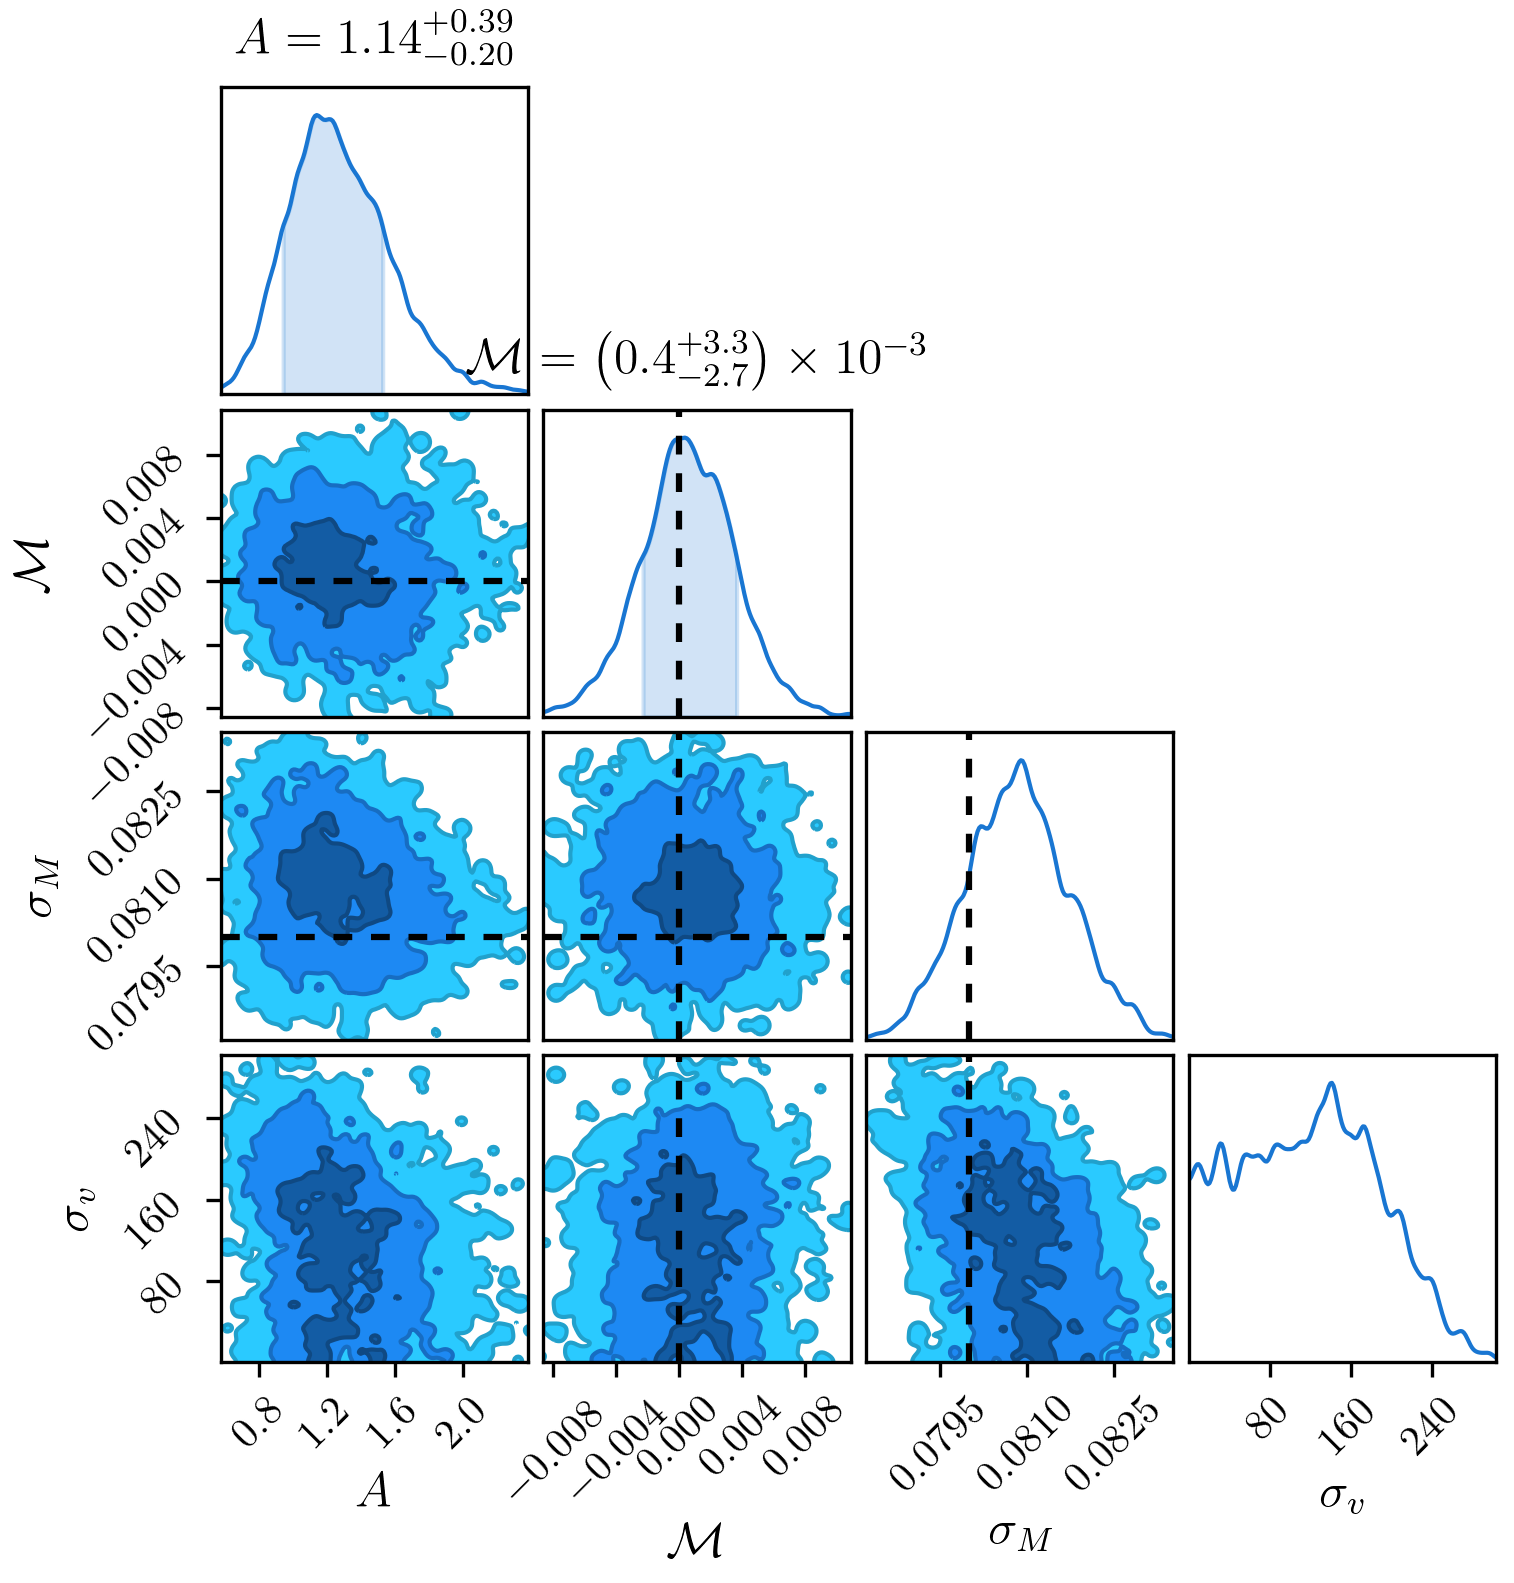
\includegraphics[width=0.5\textwidth]{../outcosmo/pvlist.0.08.1234.0.65.0.2.pkl.png}
\caption{Confidence regions for the model parameters.  $A=(f\sigma_8)/(f\sigma_8)_{GR}$, $\mathcal{M}$ is the supernova
absolute magnitude, $\sigma_M$ is the magnitude dispersion, and $\sigma_v$ is the non-linear contribution
to peculiar velocity.  This result is for the subset $z_{max}=0.2$, $\sigma_M=0.08$, $\phi=0.65$.  The dotted lines represent the inputs of the supernova
part of the simulation.
\label{zmax:fig}}
\end{figure}

\begin{table}
   \centering
   %\topcaption{Table captions are better up top} % requires the topcapt package
   \begin{tabular}{|ccc|cc|} % Column formatting, @{} suppresses leading/trailing space
   \hline
$z_{max}$ & $\phi$ & $\sigma_{M}$  &  STON $f\sigma_8$ & STON per SN \\
\hline
0.07 & 0.65 & 0.08  & 25.795 &   0.27 \\
0.07 & 1.00 & 0.08  & 31.163 &   0.27 \\
0.07 & 1.00 & 0.10  & 25.421 &   0.22 \\
0.07 & 1.00 & 0.12  & 22.173 &   0.19 \\
0.07 & 1.00 & 0.15  & 18.831 &   0.16 \\
0.10 & 0.30 & 0.08  & 23.784 &   0.24 \\
0.10 & 0.50 & 0.08  & 23.501 &   0.18 \\
0.10 & 0.65 & 0.08  & 24.994 &   0.17 \\
0.10 & 0.65 & 0.10  & 20.866 &   0.15 \\
0.10 & 0.65 & 0.12  & 18.778 &   0.13 \\
0.10 & 1.00 & 0.08  & 31.704 &   0.18 \\
0.10 & 1.00 & 0.10  & 25.687 &   0.15 \\
0.10 & 1.00 & 0.12  & 22.982 &   0.13 \\
0.15 & 0.30 & 0.08  & 24.799 &   0.15 \\
0.15 & 0.30 & 0.12  & 19.527 &   0.12 \\
0.15 & 0.50 & 0.08  & 29.550 &   0.14 \\
0.15 & 0.65 & 0.08  & 33.921 &   0.14 \\
0.15 & 0.65 & 0.10  & 28.655 &   0.12 \\
0.15 & 0.65 & 0.12  & 24.111 &   0.10 \\
0.15 & 1.00 & 0.08  & 40.158 &   0.13 \\
0.20 & 0.20 & 0.08  & 26.487 &   0.12 \\
0.20 & 0.30 & 0.08  & 29.828 &   0.11 \\
0.20 & 0.30 & 0.10  & 24.019 &   0.09 \\
0.20 & 0.30 & 0.12  & 19.181 &   0.07 \\
0.20 & 0.50 & 0.08  & 36.680 &   0.11 \\
0.20 & 0.65 & 0.08  & 41.591 &   0.11 \\
0.20 & 0.65 & 0.10  & 35.196 &   0.09 \\
0.20 & 0.65 & 0.12  & 27.987 &   0.07 \\
0.20 & 1.00 & 0.08  & 48.368 &   0.10 \\
0.20 & 1.00 & 0.10  & 40.835 &   0.08 \\
0.20 & 1.00 & 0.12  & 37.875 &   0.08 \\
    \hline
   \end{tabular}
   \caption{ston in $A$ or equivalently $f\sigma_8$ for surveys parameterized by the maximum redshift $z_{max}$,
   the fraction of total supernovae in 10 years ``fraction'', intrinsic magnitude dispersion $\sigma_{SN}$.  The number of galaxies
   $N_{gal}$, the signal $\bar{A}$ and its uncertainty $\sigma_A$ are for the cosmoDC2 (v1.0) 760 sq.~deg. volume only.
   The uncertainty ``per'' supernova is given by  $\sigma_A N_{gal}^{-0.5}$.  The ston, scaled to an LSST solid angle, is given as 
    $\bar{A} \sigma_A^{-1} (18000/760)^{0.5}$.
   \label{tab:subsets}}
\end{table}

In Fourier space, the data covariance is a combination of sample and shot noise (Eq.~\ref{cov:eq}).
In Figure~\ref{scaling:fig} the effective LSST ston is plotted as a function of input $n \sigma^{-2}_M$ for different $z_{max}$.
For all cases, the ston improves with larger $n \sigma^{-2}_M$ showing that the sample-variance limit has not been reached,
though the shallowing of the slopes for shallower surveys shows that it does contribute non-negligibly.
The fact that the ston is not constant indicates that not of the subsamples is sample-variance limited, though its non-linearity
indicates that it is non-negligible.


\begin{figure}
\centering
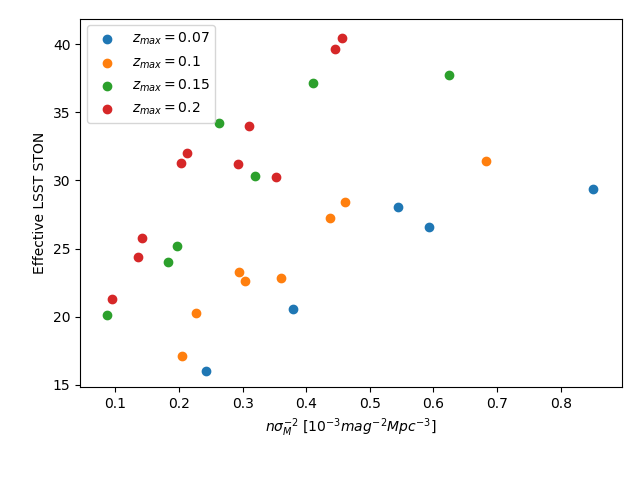
\includegraphics[width=0.5\textwidth]{../outcosmo/fracsnsig2_.png}
%\includegraphics[width=0.5\textwidth]{../outcosmo/zmax_.png}
\caption{ Effective LSST ston as a function of input  $n \sigma^{-2}_M$.  The points are color-coded for different $z_{max}$.
\label{scaling:fig}}
\end{figure}

A SN peculiar survey benefits from greater redshift depth $z_{max}$ due to the increase in volume and numbers of supernovae.  However,  for fixed magnitude uncertainty
peculiar-velocity uncertainties increase with redshift and the follow-up of fainter distant SNe requires more resources. 
Table~\ref{tab:subsets}
shows that the effective worth of each supernova ($\sigma_A N_{gal}^{-0.5}$) diminishes with increasing survey depth.
The table also shows that for $\sigma_M=0.08$~mag, the subsample with $z_{max}=0.1$ with 1294 supernovae yields a ston of 15.96, whereas
a sample with $z_{max}=0.2$ with 2021 supernovae has a lower ston of 13.61.  Within the range of surveys considered, a lower-redshift supernova
is more valuable than one at high redshift.  For both scientific and resource reasons, it is best to devote resources to the lowest possible redshifts.


$\phi \sim 0.65$ is an effective number density of discovered supernovae with light-curve coverage observed in 10 years

%
%
%\citet{2017ApJ...847..128H} project how well peculiar velocity surveys can measure $f\sigma_8$. 
%They perform their analysis in Fourier space, 
%where the Fisher information matrix of parameters $\lambda_i$ from random Gaussian field with mean zero and covariance $C(k)$ is
%\begin{equation}
%F_{ij} = \frac{V}{2}\int \frac{d^3k}{(2\pi)^3} \text{Tr}\left[ C^{-1} \frac{\partial C}{\partial \lambda_i} C^{-1}
%\frac{\partial C}{\partial \lambda_j} \right],
%\end{equation}
%where the covariance for the velocity-velocity correlation
%\begin{equation}
%C = P_{vv}(k,\mu) + \frac{\sigma^2}{n}
%\label{cov:eq}
%\end{equation}
%is dependent on the power spectrum, noise in the velocity measurement dominated by the intrinsic velocity dispersion $\sigma$, and the density of velocity probes
%\citep{2017MNRAS.464.2517H}.  
%The primary dependence on the growth of structure is through the normalization of the velocity power spectrum, such that 
%\begin{equation}
% \frac{\partial P_{vv}}{\partial \lambda} = \text{constant}
%\end{equation}
%for the parameter choice
%$\lambda=(f\sigma_8)^2$.  In the sample-variance limit, $F_{\lambda \lambda} \propto V$ whereas in the shot noise limit $F_{\lambda \lambda} \propto V n^2 \sigma^{-4}$.
%

\end{comment}

\bibliographystyle{aasjournal}
\bibliography{/Users/akim/Documents/alex}

\end{document}  